\documentclass[12pt,a4paper]{report}

%\includeonly{cover/cimlap, chapters/1_introduction}

\usepackage{styles/dolgozat}

% programkód beillesztéséhez
\usepackage{listings}

% listing float neve
\renewcommand{\lstlistingname}{Programkód}
%\renewcommand{\lstlistlistingname}{Programkódok listája}
%saját listings style-ok, és a style-t használó parancsok definíciói
\usepackage{styles/cpp}
\usepackage{styles/python}
\usepackage{styles/javascript}
%\usepackage{styles/java}
%\usepackage{styles/rust}

%% egyéb csomagok betöltése itt, vagy a dolgozat.sty fájlban

\usepackage{hyperref}
\usepackage{enumitem}
% cleveref csomag és beállításai -- az egyetlen, amit a hyperref után kell betölteni!
\usepackage{styles/refs}

\begin{document}

\pagestyle{empty}
\pagenumbering{gobble}

\pagestyle{empty} %a címlapon ne legyen semmi=empty, azaz nincs fejléc és lábléc

% A Miskolci Egyetem címere
{\large
    \begin{center}
        \vglue 1truecm
        \textbf{\huge\textsc{Szakdolgozat}}\\
        \vglue 1truecm
        
\includegraphics[width=4.8truecm, height=4truecm]{images/me_logo.png}\\
        \textbf{\textsc{Miskolci Egyetem}}
    \end{center}}

\vglue 1.5truecm %függõleges helykihagyás

    % A szakdolgozat címe, akár több sorban is
    {\LARGE
        \begin{center}
            \textbf{Közösségi Videómegosztó Szoftver Tervezése és Implementálása}
        \end{center}}

\vspace*{2.5truecm}
% A hallgató neve, évfolyam, szak(ok), a konzulens(ek) neve
{\large
    \begin{center}
        \begin{tabular}{c}
            \textbf{Készítette:}   \\
            Nagy Máté \\
            Programtervez\H o Informatikus
        \end{tabular}
    \end{center}
    \begin{center}
        \begin{tabular}{c}
            \textbf{Témavezető:} \\
            Fazekas Levente \'Aron
        \end{tabular}
    \end{center}}
\vfill
% Keltezés: Hely, év
{\large
    \begin{center}
        \textbf{\textsc{Miskolc, 2024}}
    \end{center}}

\newpage
%Feladatkiiras
\noindent
\textsc{\textbf{Miskolci Egyetem}}\\
Gépészmérnöki és Informatikai Kar\\
Alkalmazott Matematikai Intézeti Tanszék\hspace*{4cm}\hfil \textbf{Szám:}

\vspace{0.5cm}
\begin{center}
    \large\textsc{\textbf{Szakdolgozat Feladat}}
\end{center}
\vspace{0.5cm}
\textbf{Nagy Máté} (U3ROFS) programtervező informatikus jelölt részére.

\bigskip
\noindent\textbf{A szakdolgozat tárgyköre:} Webtechnológiák

\bigskip
\noindent\textbf{A szakdolgozat címe:} Közösségi Videómegosztó Szoftver Tervezése és Implementálása

\bigskip
\noindent\textbf{A feladat részletezése:}
\begin{enumerate}
    \item A szakdolgozat célja egy valós idejű videómegosztásra alkalmas webes applikáció tervezése és implementálása.
    \item Mutassa be a WebSocket és egyéb webes, valós idejű kommunikációra alkalmas API-kat!
    \item Tervezzen meg \'es implement\'aljon egy szoftvert, amely k\'epes az al\'abbi funkci\'ok elvégzésére:
          \begin{enumerate}
              \item Felhasználós nyilvántartása
              \item Videómegosztásra alkalmas szobák létrehozása, nyilvántartása
              \item Egyidejű vetítés azonos szobában tartózkodó felhasználók számára
              \item Felhasználók közötti chat
          \end{enumerate}
    \item Mutassa be az esetleges tov\'abbfejleszt\'esi lehet\H os\'egeket!
\end{enumerate}

\medskip

\vfill

\noindent\textbf{Témavezető:} Fazekas Levente \'Aron (tansz\'eki m\'ern\"ok)

% \noindent\textbf{Konzulens(ek):} (akkor kötelezõ, ha a témavezetõ nem valamelyik matematikai tanszékrõl való; de persze lehet egyébként is)\newline

\bigskip
\noindent\textbf{A feladat kiadásának ideje:} 2023.09.01.

\noindent\textbf{A feladat beadásának határideje:}

\vspace{1.5cm}

\hfill\makebox[6cm]{\dotfill}

\hfill\makebox[6cm]{szakfelelős}

\clearpage

\vspace*{1cm}
\begin{center}
    \large\textsc{\textbf{Eredetiségi Nyilatkozat}}
\end{center}
\vspace*{2cm}

Alulírott \textbf{Nagy Máté}; Neptun-kód: \texttt{U3ROFS} a Miskolci Egyetem Gépészmérnöki és Informatikai Karának végzős Programtervező informatikus szakos hallgatója ezennel büntetőjogi és fegyelmi felelősségem tudatában nyilatkozom és aláírásommal igazolom, hogy \textit{Közösségi Videómegosztó Szoftver Tervezése és Implementálása}
című szakdolgozatom saját, önálló munkám; az abban hivatkozott szakirodalom
felhasználása a forráskezelés szabályai szerint történt.

\medskip
Tudomásul veszem, hogy szakdolgozat esetén plágiumnak számít:
\begin{itemize}
    \item szószerinti idézet közlése idézőjel és hivatkozás megjelölése nélkül;
    \item tartalmi idézet hivatkozás megjelölése nélkül;
    \item más publikált gondolatainak saját gondolatként való feltüntetése.
\end{itemize}

Alulírott kijelentem, hogy a plágium fogalmát megismertem, és tudomásul veszem, hogy
plágium esetén szakdolgozatom visszautasításra kerül.

\vspace*{3cm}

\noindent Miskolc, \makebox[2cm]{\dotfill}. év \makebox[2cm]{\dotfill}. hó \makebox[2cm]{\dotfill}. nap

\vspace*{3cm}

\hfill\makebox[6cm]{\dotfill}

\hfill\makebox[6cm]{Hallgató}



\clearpage

\newcommand{\ki}{témavezető(k)}
\newsavebox{\alairas}
\begin{lrbox}{\alairas}
    \begin{tabular}{c@{\hspace{2cm}}c}
        \makebox[4cm]{\dotfill} & \makebox[5cm]{\dotfill} \\
        dátum                   & \ki                     \\
    \end{tabular}
\end{lrbox}
\newcommand{\dotline}{\makebox[5cm]{\dotfill}}
\newcommand{\shortdotline}{\makebox[3.5cm]{\dotfill}}

\noindent 1.
\begin{tabular}[t]{cl}
    \multirow{2}{*}{A szakdolgozat feladat módosítása}
     & szükséges (módosítás külön lapon) \\
     & nem szükséges                     \\[1ex]
\end{tabular}

\begin{center}
    \usebox{\alairas}
\end{center}

\smallskip

\noindent 2. A feladat kidolgozását ellenőriztem:

\begin{center}
    \begin{tabular}{c@{\hspace*{2cm}}c}
        témavezető (dátum, aláírás): & konzulens (dátum, aláírás): \\
        \dotline                     & \dotline                    \\
        \dotline                     & \dotline                    \\
        \dotline                     & \dotline
    \end{tabular}
\end{center}

\smallskip

\noindent 3. A szakdolgozat beadható:

\begin{center}
    \usebox{\alairas}
\end{center}

\noindent 4.
\begin{tabular}[t]{@{}l@{\hspace*{1mm}}l@{\hspace*{1mm}}l}
    A szakdolgozat & \shortdotline & szövegoldalt                                      \\
                   & \shortdotline & program protokollt (listát, felhasználói leírást) \\
                   & \shortdotline & elektronikus adathordozót (részletezve)           \\
                   & \shortdotline                                                     \\
                   & \shortdotline & egyéb mellékletet (részletezve)                   \\
                   & \shortdotline
\end{tabular}
\newline tartalmaz.

\begin{center}
    \usebox{\alairas}
\end{center}

\noindent 5.
\begin{tabular}[t]{ll}
    \multirow{2}{*}{A szakdolgozat bírálatra} & bocsátható     \\
                                              & nem bocsátható \\
\end{tabular}

\smallskip

\noindent A bíráló neve: \makebox[8cm]{\dotfill}

\renewcommand{\ki}{szakfelelős}
\begin{center}
    \begin{tabular}{c@{\hspace{2cm}}c}
        \makebox[4cm]{\dotfill} & \makebox[5cm]{\dotfill} \\
        dátum                   & \ki                     \\
    \end{tabular}
\end{center}

\noindent 6.
\begin{tabular}[t]{lll}
    A szakdolgozat osztályzata                                        \\
     & a témavezető javaslata:            & \makebox[2.5cm]{\dotfill} \\
     & a bíráló javaslata:                & \makebox[2.5cm]{\dotfill} \\
     & a szakdolgozat végleges eredménye: & \makebox[2.5cm]{\dotfill}
\end{tabular}

\bigskip\bigskip

\noindent Miskolc, \makebox[4cm]{\dotfill} \hfill \makebox[8cm]{\dotfill}

\hfill \makebox[8cm]{a Záróvizsga Bizottság Elnöke}


\tableofcontents

\clearpage
\pagenumbering{arabic}
\pagestyle{fancy}

\chapter{Bevezetés}\label{chapter:bevezetes}
A digitális korban élünk, ahol a technológia gyorsan fejlődik
és az embereknek egyre több lehetőségük van az online interakcióra.
Azonban a közösségi médiával és az egyéb digitális platformokkal eltöltött
idő gyakran személytelen és egyoldalú.

A "WatchWithFriends" névre keresztelt alkalmazásom arra hivatott,
hogy ezen változtasson. Az alkalmazás lehetőséget nyújt arra,
hogy a felhasználók együtt nézzenek YouTube-videókat, miközben élő chaten
kommunikálnak egymással.
Az alkalmazásban létrehozott "szobák" révén a felhasználók egyszerűen csatlakozhatnak,
és megoszthatják egymással kedvenc videóikat egy közös lejátszási listán keresztül.
Az alkalmazás nem csupán egy online videómegosztó platformot egészít ki,
hanem egy új közösségi élményt is kínál. Ezzel az eszközzel a barátok és családok,
akár távoli földrészeken is, összehozhatók egy közös élmény kapcsán. A "WatchWithFriends" az együtt töltött idő minőségét kívánja javítani, lehetővé téve, hogy az emberek valós időben osszák meg reakcióikat, érzéseiket egy-egy videóval kapcsolatban.

Továbbá a chat funkcióval a felhasználók azonnal megvitathatják a látottakat,
megoszthatják tippeiket vagy akár következő videó választási ötleteiket is.

A szoftver nem csak szórakoztató, de oktatási célokra is felhasználható.
Tanárok és diákok könnyedén nézhetnek együtt oktatási anyagokat, és azonnal megbeszélhetik azok tartalmát.
Ezen kívül a vállalati prezentációknál is hasznos lehet a közös videómegtekintés funkció.

A "WatchWithFriends" egy olyan platform, ami a társasági interakciókat nem csak kiterjeszti,
de egy új dimenzióba is emeli. Az alkalmazás tehát nem csak egy technológiai újítás, hanem egy közösségi eszköz is, amely összeköti az embereket függetlenül fizikai távolságuktól.
\chapter{Tervez\'es}\label{chapter:tervezes}

\section*{Átfogó struktúra}
Az alkalmazásom két részből áll, a kliens oldali és a szerver oldali részből.
A kliens oldali rész a felhasználói felületet valósítja meg, a szerver oldali rész pedig az üzleti logikát, és az adatbázis kezelést.
\\
\subsection*{Kliens-oldal}
A kliens oldal felelős a felhasználói interakciókért és a felhasználói felület megjelenítéséért. Itt találhatók a gombok, formok, és egyéb elemek, amikkel a felhasználók közvetlenül érintkeznek. A kliens oldalon futó kód gyakran aszinkron módon kommunikál a szerverrel, hogy adatokat kérjen vagy küldjön.
\\
\subsection*{Szerver-oldal}
A szerver oldal felelős a kliens oldal által küldött kérések feldolgozásáért, és a válaszok generálásáért. Itt található az üzleti logika, és az adatbázis kezelés. A szerver oldali kód futása általában szinkron módon történik, és a kliens oldali kérések feldolgozása után küldi a válaszokat.
\begin{figure}[H]
    \centering
    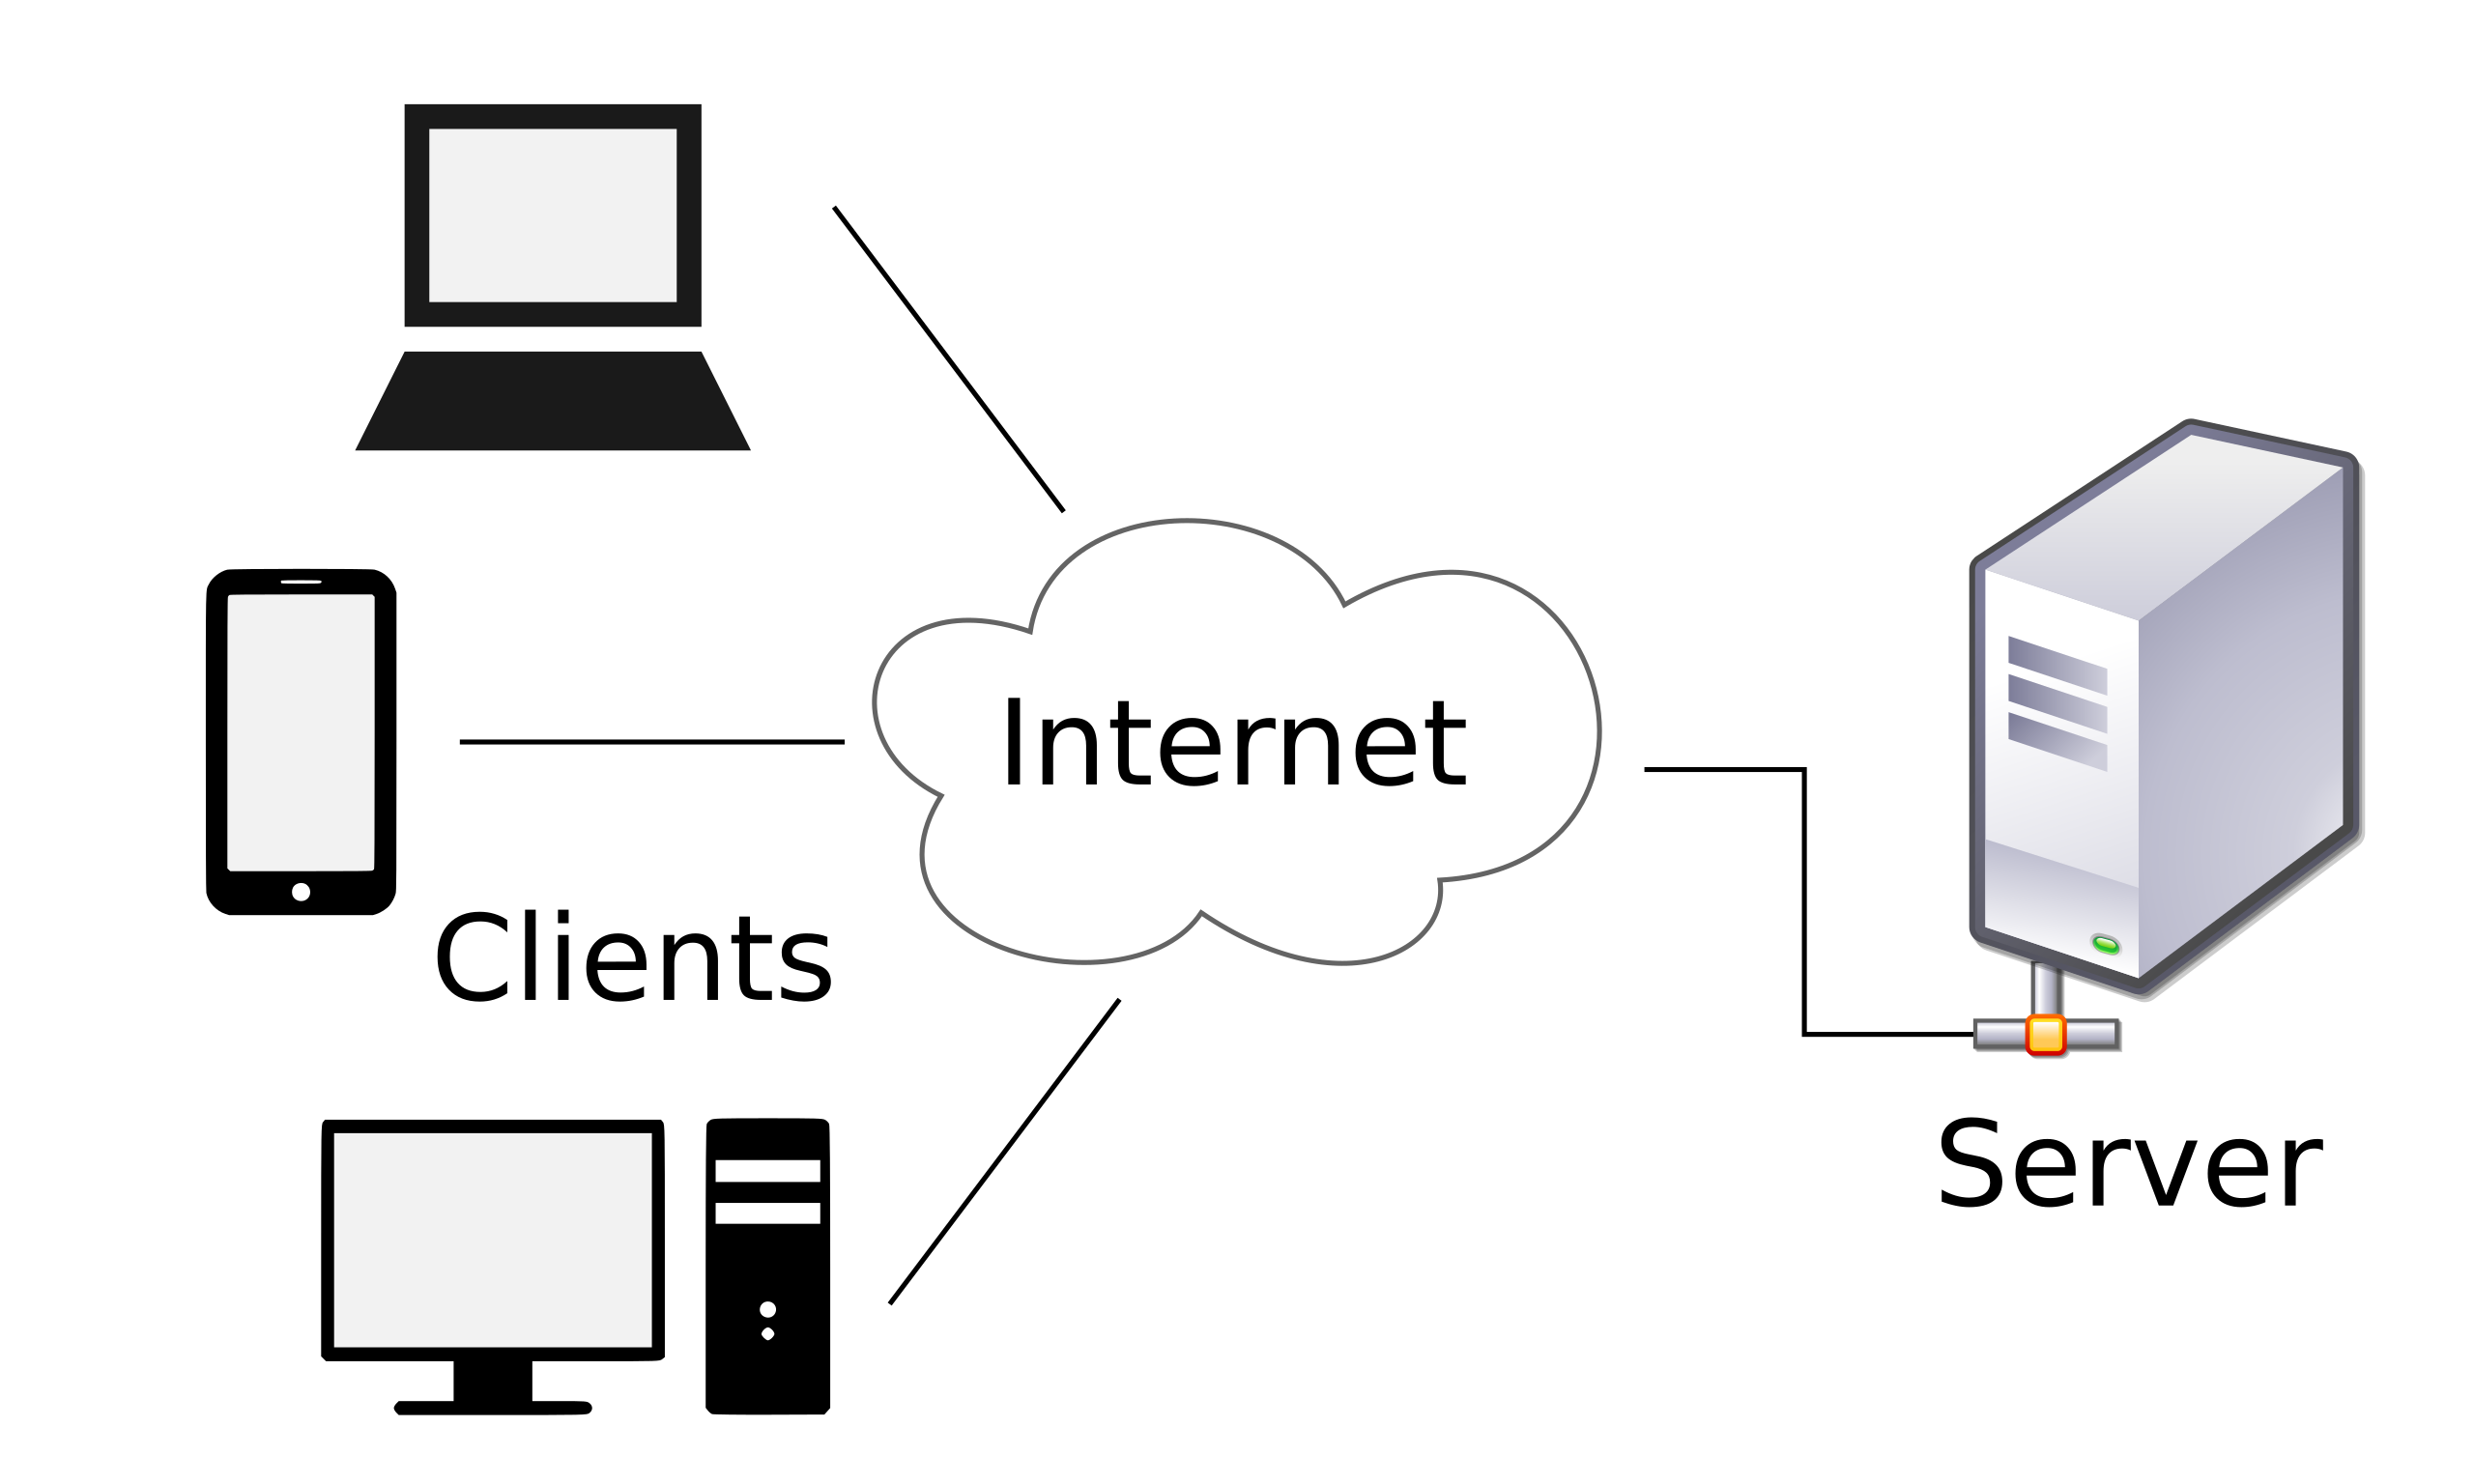
\includegraphics[width=14.0truecm]{images/Client-server-model.png}
    \caption[Átfogó struktúra]{Átfogó struktúra \cite{architecture}}
    \label{fig:architecture}
\end{figure}

\section*{Kliens oldali logika}
A kliens oldali logikát a következő architektúra alapján terveztem meg.
\begin{figure}[H]
    \centering
    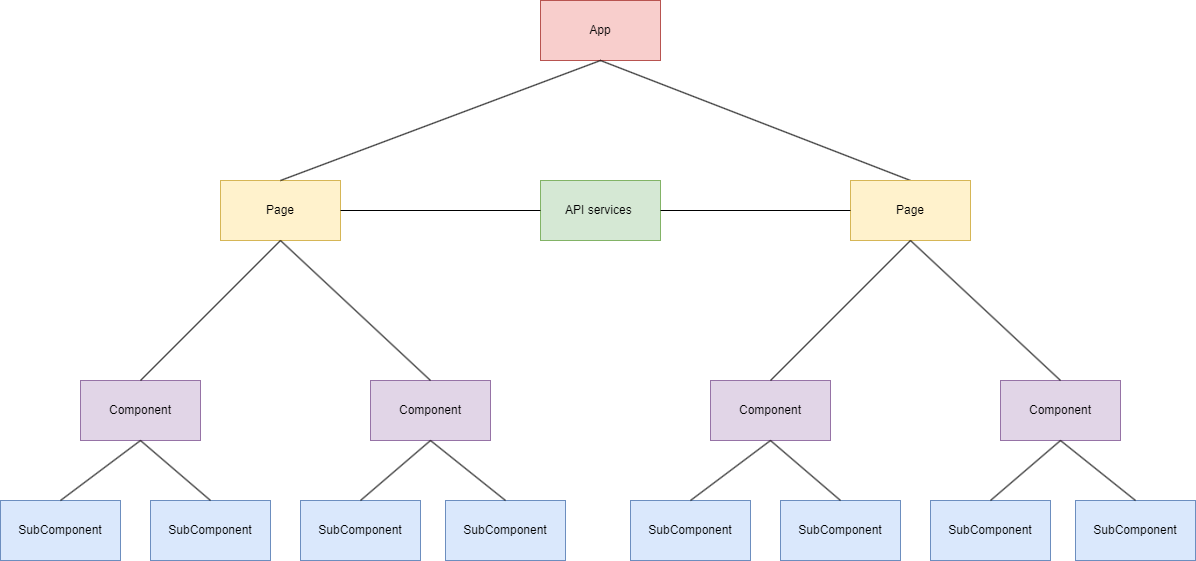
\includegraphics[width=14.0truecm]{images/Frontend_architecture.png}
    \caption{Frontend Architektúra}
    \label{fig:frontend_architecture}
\end{figure}
A fejlesztés során törekedtem a komponensek újra felhasználhatóságára, és a kód minél jobb strukturáltságára.
\\
\textbf{Ismertetem a komponensek főbb tulajdonságait:}
\begin{itemize}
    \item \textbf{App:} Az alkalmazás gyökér komponense. Itt található a Router, amely a különböző útvonalakhoz rendeli a megfelelő komponenseket.
    \item \textbf{Page:} Az alkalmazás View komponensei. A különböző oldalakat reprezentálják. Itt találhatóak a különböző komponensek, amelyek a megjelenítést végzik. Illetve itt használom az API hívásokat is.
    \item \textbf{API services:} Itt találhatóak a különböző API végpontokat kezelő függvények.
    \item \textbf{Component:} Az alkalmazás nagyobb komponensei. Ezek a komponensek több kisebb komponensből állnak össze.
    \item \textbf{SubComponent:} Az alkalmazás kisebb komponensei. Ezek a komponensek csak egy adott feladatot látnak el.
\end{itemize}


\section*{Szerver oldali logika}
\subsection*{Architektúra}
Az alkalmazásnál MVC (Model-View-Controller) architektúrára építettem, illetve
bővítettem a Repository és a Service rétegekkel. Az MVC architektúra egy
architektúrális minta, amely a felhasználói felületet (View), az alkalmazás
logikáját (Controller) és az adatokat (Model) három különálló részre osztja.
A Repository réteg a Model réteghez tartozik, a Service réteg pedig a Controller réteghez.
Azért bontottam tovább a rétegeket, mert így jobban elkülönülnek a felelősségi körök,
és a kód is átláthatóbb lesz, illetve könnyebben bővíthető, és tesztelhető lesz.
\\
\\
\begin{figure}[H]
    \centering
    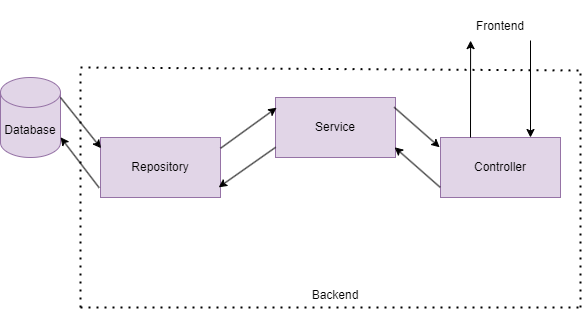
\includegraphics[width=14.0truecm]{images/Backend_architecture.png}
    \caption{Backend Architektúra}
    \label{fig:backend_architecture}
\end{figure}
\textbf{Ismertetem a rétegek főbb tulajdonságait:}
\begin{itemize}
    \item \textbf{Adatbázis}: Az alkalmazásom adattára. Itt tárolódnak a statikus és dinamikus adatok.
    \item \textbf{Repositoryk}: Az adatbázis és az alkalmazás logikája közötti köztes réteg. CRUD műveletek, komplex lekérdezések.
    \item \textbf{Servicek}: Az üzleti logika helye. Itt történnek a komplex számítások, validációk és egyéb logikai műveletek.
    \item \textbf{Controllerek}: Az API végpontokat kezelő réteg. Fogadják a kliens kéréseit, és válaszokat generálnak.
\end{itemize}

\section*{Adatbázis}
\subsection*{ER modell egyedei és tulajdonságai}
\textbf{User-ek tulajdonságai:}
\begin{itemize}
    \item \underline{Id}: Elsődleges kulcs, Guid típusú.
    \item \underline{Name}: Felhasználó neve, szöveg típusú.
    \item \underline{Email}: Felhasználó email címe, szöveg típusú.
    \item \underline{PasswordHash}: Felhasználó jelszavának hash-elt változata, szöveg típusú.
    \item \underline{Salt}: Felhasználó jelszavának sója, szöveg típusú.
    \item \underline{BirthDate}: Felhasználó születési dátuma, dátum típusú.
\end{itemize}
\textbf{Image-ek tulajdonságai:}
\begin{itemize}
    \item \underline{Id}: Elsődleges kulcs, Guid típusú.
    \item \underline{Data}: Kép binárisa, byte tömb típusú.
\end{itemize}
\textbf{Room-ok tulajdonságai:}
\begin{itemize}
    \item \underline{Id}: Elsődleges kulcs, Guid típusú.
    \item \underline{Name}: Szoba neve, szöveg típusú.
    \item \underline{CreatorId}: Tulajdonos azonosítója, Guid típusú.
    \item \underline{CreationTime}: Szoba létrehozásának ideje, dátum típusú.
    \item \underline{CurrentVideoId}: Jelenleg lejátszott videó azonosítója, Guid típusú.
    \item \underline{PasswordHash}: Szoba jelszavának hash-elt változata, szöveg típusú.
    \item \underline{Salt}: Szoba jelszavának sója, szöveg típusú.
\end{itemize}
\textbf{Video-k tulajdonságai:}
\begin{itemize}
    \item \underline{Id}: Elsődleges kulcs, Guid típusú.
    \item \underline{Title}: Videó címe, szöveg típusú.
    \item \underline{Url}: Videó URL-je, szöveg típusú.
    \item \underline{ThumbnailURL}: Videó thumbnail-je, szöveg típusú.
\end{itemize}

\begin{figure}[H]
    \centering
    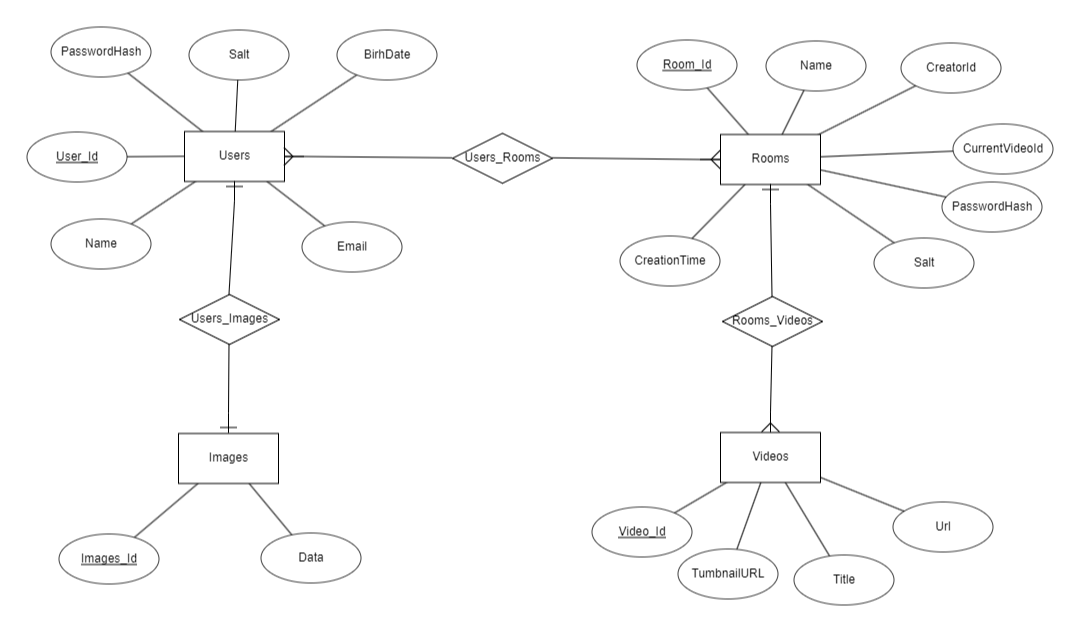
\includegraphics[width=15.0truecm]{images/er_modell.png}
    \caption{ER modell}
    \label{fig:er_modell}
\end{figure}

\subsection*{Relációs modell}
\textbf{Az egyedek közötti kapcsolatok:}
\begin{itemize}
    \item \underline{Users-Images}: 1:1 Egy felhasználóhoz tartozhat egy kép, és a kép csak egy fel-
          használóhoz.
    \item \underline{Users-Rooms}: N:N Egy felhasználóhoz tartozhat több szoba, egy szoba is tartozhat
          több felhasználóhoz.
    \item \underline{Room-Video}: 1:N Egy szobához tartozhat több videó, de egy videó csak egy
          szobához tartozhat.
\end{itemize}

\begin{figure}[H]
    \centering
    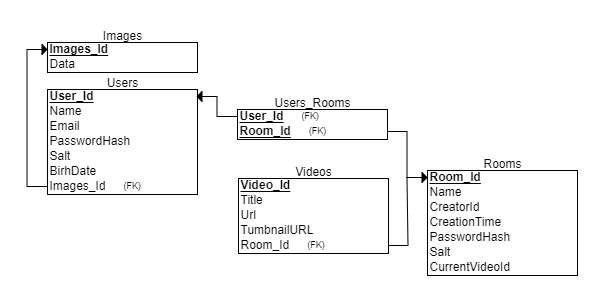
\includegraphics[width=15.0truecm]{images/relation_modell.png}
    \caption{Relációs modell}
    \label{fig:relation_modell}
\end{figure}

\subsection*{Szoftvertervezési elvek}
A szoftvertervezési elvek alapvető útmutatások a kiváló kód fejlesztéséhez. Ezek az iránymutatások növelik a kód minőségét, gyorsítják a fejlesztési folyamatot és minimalizálják a hibalehetőségeket. Az ilyen elvek segítenek abban, hogy a kód könnyen újrafelhasználható és karbantartható legyen.

A kód olvashatóságát és tesztelhetőségét is javítják, ami hosszú távon időt és erőforrást spórol. A rugalmasság és a bővíthetőség is nő, tehát a kód könnyen adaptálható új funkciók vagy változások esetén. Továbbá, ezek az elvek ösztönzést nyújtanak a kódbázis redundancia kiküzsöbölésére, amely csökkenti a komplexitást és növeli a kohéziót. Az elvek célja a kód moduláris felépítése és az alacsonyabb összekapcsoltság, ami hozzájárul a jobb szervezettséghez és könnyebb karbantartáshoz.

Összességében, a szoftvertervezési elvek olyan iránymutatások, amelyek célja a hatékony, karbantartható és minőségi kód létrehozása.
A szoftver implementációja során a SOLID elveket vettem alapul.

\section*{UML diagram}

\begin{figure}[H]
    \centering
    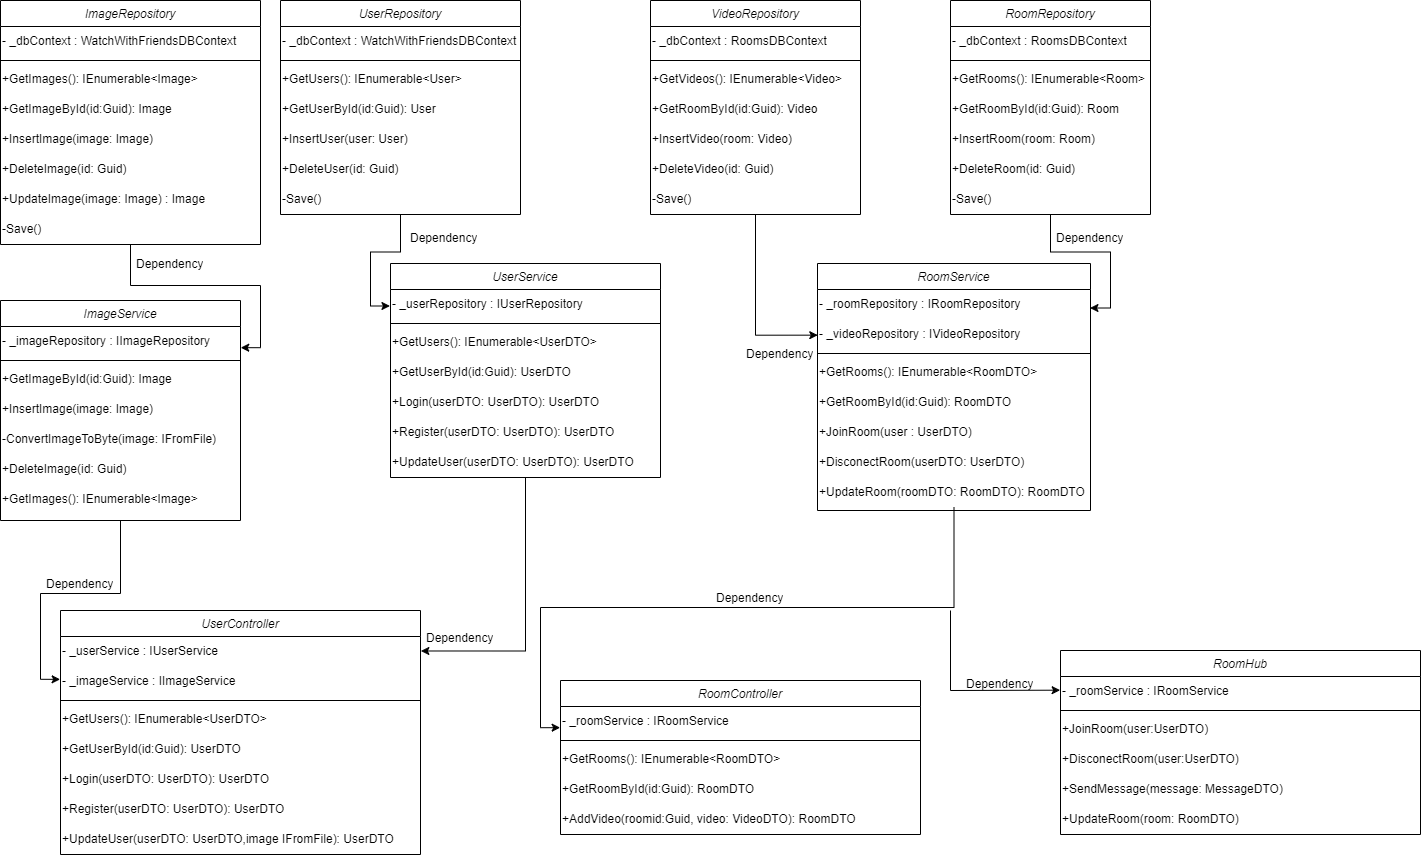
\includegraphics[width=14.0truecm]{images/UML_Diagram.png}
    \caption{UML Diagram}
    \label{fig:uml_diagram}
\end{figure}

Az architektúra alapját egy kibővített MVC (Model-View-Controller) rendszer adja,
amely kifinomult kapcsolatokat biztosít az egyes szerveroldali osztályok között. Mivel a back-end és a front-end kapcsolata indirekt,
ezért a megjelenítési oldalon található logika nincs semmilyen ráhatással a szerver struktúrális felépítésére.
Ebben az elrendezésben az egyes osztályok nem csak az alapvető CRUD (Create,
Read, Update, Delete) műveletekért felelnek, hanem a komplex üzleti logika egyedi
implementációját is lehetővé teszik. Az adatmodell és a kontroller között az adatátviteli objektumok (DTO-k) és a repository minták segítenek a moduláris és tiszta kód

struktúra fenntartásában. A repository-k pedig közvetlenül a dedikált adatbázis-kontextusokhoz kapcsolódnak.

A kapcsolatok közötti szoros integráció lehetővé teszi az adatok egyszerű és követke-
zetes kezelését, miközben fenntartja a kód karbantarthatóságát és tesztelhetőségét. Az

egész rendszer ezen az elrendezésen alapul, így garantálva, hogy a szerveroldali logika
jól szervezett és hatékony maradjon.
\chapter{Technol\'ogia}\label{chapter:technologia}
\section{Felhasználói felület}
Az alkalmazás felhasználói felületét a React könyvtár segítségével valósítottam meg.
A React egy nyílt forráskódú JavaScript könyvtár, amelyet a Facebook fejlesztett ki.
A könyvtár célja, hogy a felhasználói felület fejlesztését egyszerűbbé tegye.
A React egy komponens alapú könyvtár, amely lehetővé teszi a fejlesztők számára,
hogy újra felhasználható komponenseket hozzanak létre, amelyeket összeállítva
komplex felhasználói felületeket hozhatnak létre.
\\
\\
\textbf{Komponensek}
A React komponensek egyfajta sablonok, amelyek a felhasználói felület egy részét írják le.
A komponensek egy egyszerű JavaScript objektumok, amelyeknek van egy render metódusa,
amely visszaadja a komponens felhasználói felületét.
\\
\\
\textbf{Komponensek főbb tulajdonságai:}
\begin{itemize}
    \item Paraméterek (props)
    \item Gyerekei (children)
    \item Állapotai (state)
    \item Életciklus metódusai (lifecycle)
    \item Eseménykezelői (event)
    \item Stílusai (style)
    \item Referenciák (ref)
    \item Kontextusai (context)
    \item Típusai (type)
    \item Kulcsai (key)
\end{itemize}
\subsection*{React és Angular összehasonlítása}
A front-end keretrendszer választása fontos lépése az implementáció előkészítésének. Két népszerű keretrendszer képezte a lehetőségek listáját: az Angular és a React.
\\
\\
\textbf{Különbség a React és az Angular között:}
\begin{table}[h]
    \centering
    \begin{tabular}{|l|l|l|}
        \hline
                               & React           & Angular                 \\
        \hline
        Egyszerűség            & Könnyű tanulni. & Több beépített funkció. \\
        \hline
        Flexibilitás           & Rugalmas.       & Kevesebb szabadság.     \\
        \hline
        Teljesítmény           & Virtuális DOM.  & Two-Way Data Binding.   \\
        \hline
        Ökoszisztéma           & Nagy közösség.  & Minőségi eszközök.      \\
        \hline
        Fejlesztői tapasztalat & JSX.            & TypeScript.             \\
        \hline
    \end{tabular}
    \caption[Különbségek React és Angular között]{Különbségek React és Angular között}
\end{table}
\subsection*{Redux vagy Context API}
Az alkalmazás állapotainak kezelésére több lehetőség is felmerült, közöttük a Redux és a Context API.
A Redux egy állapotkezelő könyvtár, amely lehetővé teszi az alkalmazás állapotának tárolását egy központi helyen.
A Context API egy React API, amely lehetővé teszi az alkalmazás állapotának tárolását és megosztását a komponensek között.
Mivel az alkalmazás kis méretű, ezért a Context API-ra esett a választás.
\\
\\
\textbf{A Context API főbb tulajdonságai:}
\begin{itemize}
    \item \textbf{Beépített megoldás:} A Context API része a React alapkönyvtárnak, nincs szükség külső függőségekre.
    \item \textbf{Egyszerűség:} A Context API egyszerűbb és könnyen megérthető, kevesebb boilerplate kóddal.
    \item \textbf{Nincs middleware:} Nem támogat middleware-eket alapból, így aszinkron állapotfrissítéseket manuálisan kell kezelni.
    \item \textbf{Nem optimalizált nagy alkalmazásokhoz:} Nagy alkalmazásokban hatékonytalan lehet, mert minden Context változásra újrarendereli az összes fogyasztót, hacsak nem optimalizáljuk manuálisan.
    \item \textbf{Kevesebb eszköz:} Kevesebb beépített eszköze van, mint a Redux-nak, de ez nem mindig hátrány, függ a projekt igényeitől.
\end{itemize}
\textbf{Példa a Context API állapotkezelésére:}
\begin{lstlisting}[style=es6, morekeywords={document, P5, katex},caption={Context API állapotkezelés}]
    // context
    const CounterContext = React.createContext();
    
    // state and update
    const [count, setCount] = useState(0);
    
    // state refresh
    setCount(count + 1);
\end{lstlisting}

\vspace{2em}

\textbf{A Redux főbb tulajdonságai:}
\begin{itemize}
    \item \textbf{Optimalizáció:} Redux kifejezetten optimalizált a nagyobb alkalmazások számára, és lehetővé teszi az állapot frissítéseinek finom szabályozását.
    \item \textbf{Middleware Támogatás:} Redux lehetőséget ad middleware-ek használatára, amelyek lehetővé teszik az aszinkron állapotfrissítések könnyebb kezelését.
    \item \textbf{Tesztelhetőség:} A Redux architektúrája miatt a tesztelés egyszerűbb, minden action egy független egység, és a reducer funkciók tiszta függvények.
    \item \textbf{Eszközök és Közösség:} Redux-nak nagy közössége van, és sok kiegészítő eszköz, például a Redux DevTools.
    \item \textbf{Boilerplate Kód:} Több boilerplate kód szükséges, hogy elindítsunk egy Redux-alapú állapotkezelést.
\end{itemize}
\textbf{Példa a Redux állapotkezelésére:}
\begin{lstlisting}[style=es6, morekeywords={document, P5, katex},caption={Redux állapotkezelés}]
    // action
    const incrementAction = { type: 'INCREMENT' };
    
    // reducer
    function counterReducer(state = 0, action) {
      if (action.type === 'INCREMENT') {
        return state + 1;
      }
      return state;
    }
    
    // dispatch
    dispatch(incrementAction);
\end{lstlisting}
\vspace{1em}
\subsection*{TypeScript vagy JavaScript}
A TypeScript egy nyílt forráskódú, szigorúan típusos programozási nyelv,
amely a JavaScriptre épül, lehetővé teszi a statikus típusok használatát,
és minden érvényes JavaScript kód érvényes TypeScript kódnak is számít.
Inkább a TypeScript mellett döntöttem, mert a statikus típusok használata
növeli a kód minőségét és a fejlesztési sebességet, illetve csökkenti a hiba lehetőségek számát.

\section{Szerveroldali Logika és API-k}
A szerver és a kliens közötti kommunikáció megvalósításához az ASP.NET Core-t használtam.
Az ASP.NET Core egy nyílt forráskódú, cross-platform, magas teljesítményű keretrendszer,
amelyet a Microsoft fejlesztett ki.
Az ASP.NET Core-t a webalkalmazások és a webes API-k fejlesztésére használják.
A környezetet a C\# programozási nyelvhez tervezték, de támogatja a többi .NET nyelvet is.
Én a megvalósítás során a C\# nyelvet használtam.
Ebben a fejezetben bemutatom a szerveroldali logikát és az API-kat.

\subsection*{Adatbázis}
Az alkalmazásnál MS SQL adatbázist használtam, mert a Microsoft SQL Server-t használom a személyes projekteimhez.
Az MS SQL (Microsoft SQL Server) egy relációs adatbázis-kezelő rendszer (RDBMS) a Microsofttól. Jól skálázható, és számos fejlett funkcióval rendelkezik,
mint például tárolt eljárások,
triggerek és nézetek
. Gyakran használják vállalati szintű alkalmazásokban,
és támogatja a SQL nyelvet az adatok lekérdezésére és manipulálására.
Támogatja az ACID tulajdonságokat és a tranzakciós integritást.
Az ER modell-t használtam az adatbázis tervezéséhez.
Ezt majd a Backend fejlesztési folyamatánál részletezem.

\subsection*{Entity Framework Core}
Az Entity Framework Core (EF Core) egy objektum-relációs leképzési (ORM) keretrendszer a Microsofttól,
amely .NET Core és .NET 5+ alkalmazások számára készült.
Lehetővé teszi a fejlesztők számára, hogy magas szintű,
objektumorientált API-n keresztül dolgozzanak adatbázisokkal,
anélkül hogy közvetlen SQL lekérdezéseket kellene írniuk.
Támogatja a code-first és a database-first megközelítéseket,
így rugalmasságot biztosít az adatmodell és az adatbázisséma kialakításában. Az EF Core lehetővé teszi a LINQ (Language Integrated Query) használatát,
ami természetes módon illeszkedik a C\# és más .NET nyelvekhez.

\begin{figure}[H]
    \centering
    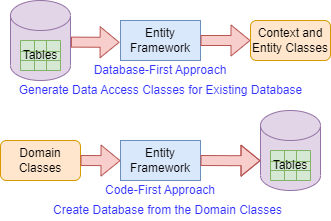
\includegraphics[width=10.0truecm]{images/EntityFramework.png}
    \caption{Entity Framework Core}
    \label{fig:entity_framework_core}
\end{figure}

Skálázható és teljesítmény-optimalizált, ezért alkalmas mind kis,
mind nagyobb vállalati projektekben. Az EF Core támogatja a többszörös adatbázis-motorokat, beleértve az SQL Server, PostgreSQL, SQLite és másokat is.
Az adatmigrációk egyszerű kezelése és automatikus generálása az egyik előnye, ami könnyebbé teszi az adatbázisséma változásainak kezelését.
A keretrendszer beépített támogatással rendelkezik a tranzakciókezelésre, így az ACID tulajdonságok biztosítottak. Az EF Core rugalmas konfigurációs lehetőségekkel rendelkezik,
és jól integrálódik más .NET Core szolgáltatásokkal, mint például a Dependency Injection. Folyamatosan fejlődik és aktívan karbantartott,
így a legújabb .NET technológiákhoz és az adatbázis-technológiákhoz is gyorsan alkalmazkodik.

\subsection*{API}
Az alkalmazásnál RESTful API-t használtam, mert a RESTful API-kat a leggyakrabban használják,
és a legtöbb fejlesztő ismeri őket. A REST (Representational State Transfer) egy architektúrális stílus,
amelyet a webes alkalmazásokhoz használnak. A RESTful API-kat a REST architektúra alapelvei alapján tervezik.
A RESTful API-kat a HTTP protokollra építik, és a HTTP metódusokat használják a kérések kezelésére.
Ennek megvalósításához a \textit{ControllerBase} osztályt használtam a Controllerekben.
Ami teljesen implementálja a RESTful API-kat, és a HTTP metódusokat.

\begin{figure}[H]
    \centering
    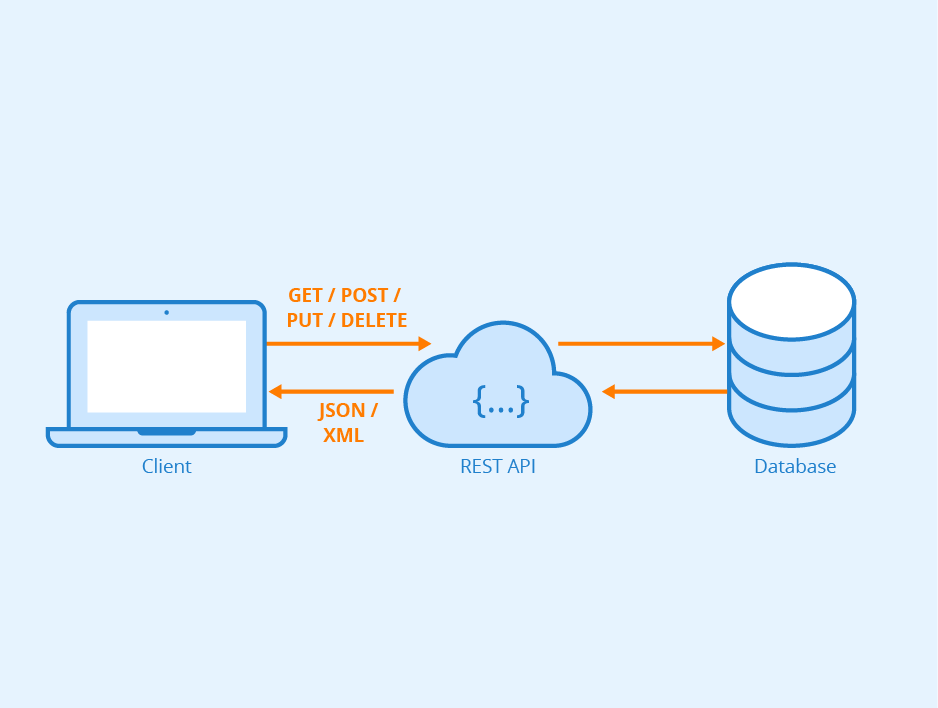
\includegraphics[width=9.0truecm]{images/Rest-API.png}
    \caption[RESTful API]{RESTful API \cite{restfulapi}}
    \label{fig:restfulapi}
\end{figure}

A videók lejátszása során különös figyelmet fordítottam
az állapotkezelésre. Ennek érdekében a WebSocket
protokollt alkalmaztam. A WebSocket egy kétirányú
kapcsolatot tesz lehetővé a böngésző és a szerver között.
Bár a HTTP protokollra épül, mégis képes valós idejű
kommunikációra. A kommunikáció HTTP portokon keresztül zajlik,
ami rugalmasságot ad az alkalmazásnak.
SignalR-t használtam a WebSocket protokoll megvalósításához.

A SignalR egy Microsoft által fejlesztett aszinkron könyvtár,
amely valós idejű webes alkalmazások építését támogatja.
Lehetővé teszi a szerver és a kliensek közötti kétirányú
kommunikációt, gyakran WebSockets használatával.

\begin{figure}[H]
    \centering
    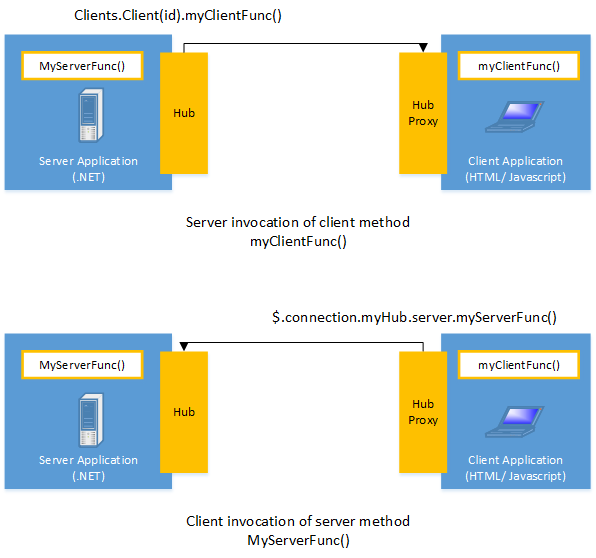
\includegraphics[width=9.0truecm]{images/SignalR.png}
    \caption[SignalR]{SignalR \cite{signalR}}
    \label{fig:signalR}
\end{figure}

Ez eltér a hagyományos HTTP "kérés-válasz" modelltől,
mivel a szerver aktívan küldhet üzeneteket a klienseknek.
Gyakori alkalmazási területei közé tartoznak a chat szolgáltatások,
online játékok és élő adatfrissítések. A SignalR automatikusan választja ki a legmegfelelőbb kommunikációs mechanizmust a szerver és a kliens között,
például long polling, ha WebSockets nem érhető el. A könyvtár könnyen integrálható más .NET technológiákkal és keretrendszerekkel, például ASP.NET Core-al.
A SignalR segítségével könnyen implementálhatók komplex forgatókönyvek, például csoportos üzenetküldés vagy kapcsolatok kezelése. Az állapotkezelés és a kiváló skálázhatóság további előnyei a SignalR használatának.
Mivel a SignalR API az ASP.NET Core része, az infrastruktúrát és a biztonsági mechanizmusokat is könnyen ki lehet terjeszteni rá. Összességében a SignalR egy erőteljes eszköz a valós idejű webes alkalmazások fejlesztéséhez.
\subsection*{Fejlesztői környezet}
Én a Visual Studio 2022-t használtam a fejlesztéshez, mert ez az egyik legnépszerűbb IDE a .NET fejlesztők körében.
A Visual Studio 2022 egy integrált fejlesztői környezet (Integrated Development Environment, IDE), amelyet a Microsoft fejlesztett ki. Ez a platform különösen népszerű a Windows alapú alkalmazások fejlesztésénél, de támogatja számos programozási nyelvet és technológiát, így a fejlesztők széles spektruma számára kínál megoldásokat. Az IDE magába foglalja a kódszerkesztést, a debuggolást, a verziókezelést és más, a fejlesztési ciklusban fontos eszközöket is.
\begin{figure}[H]
    \centering
    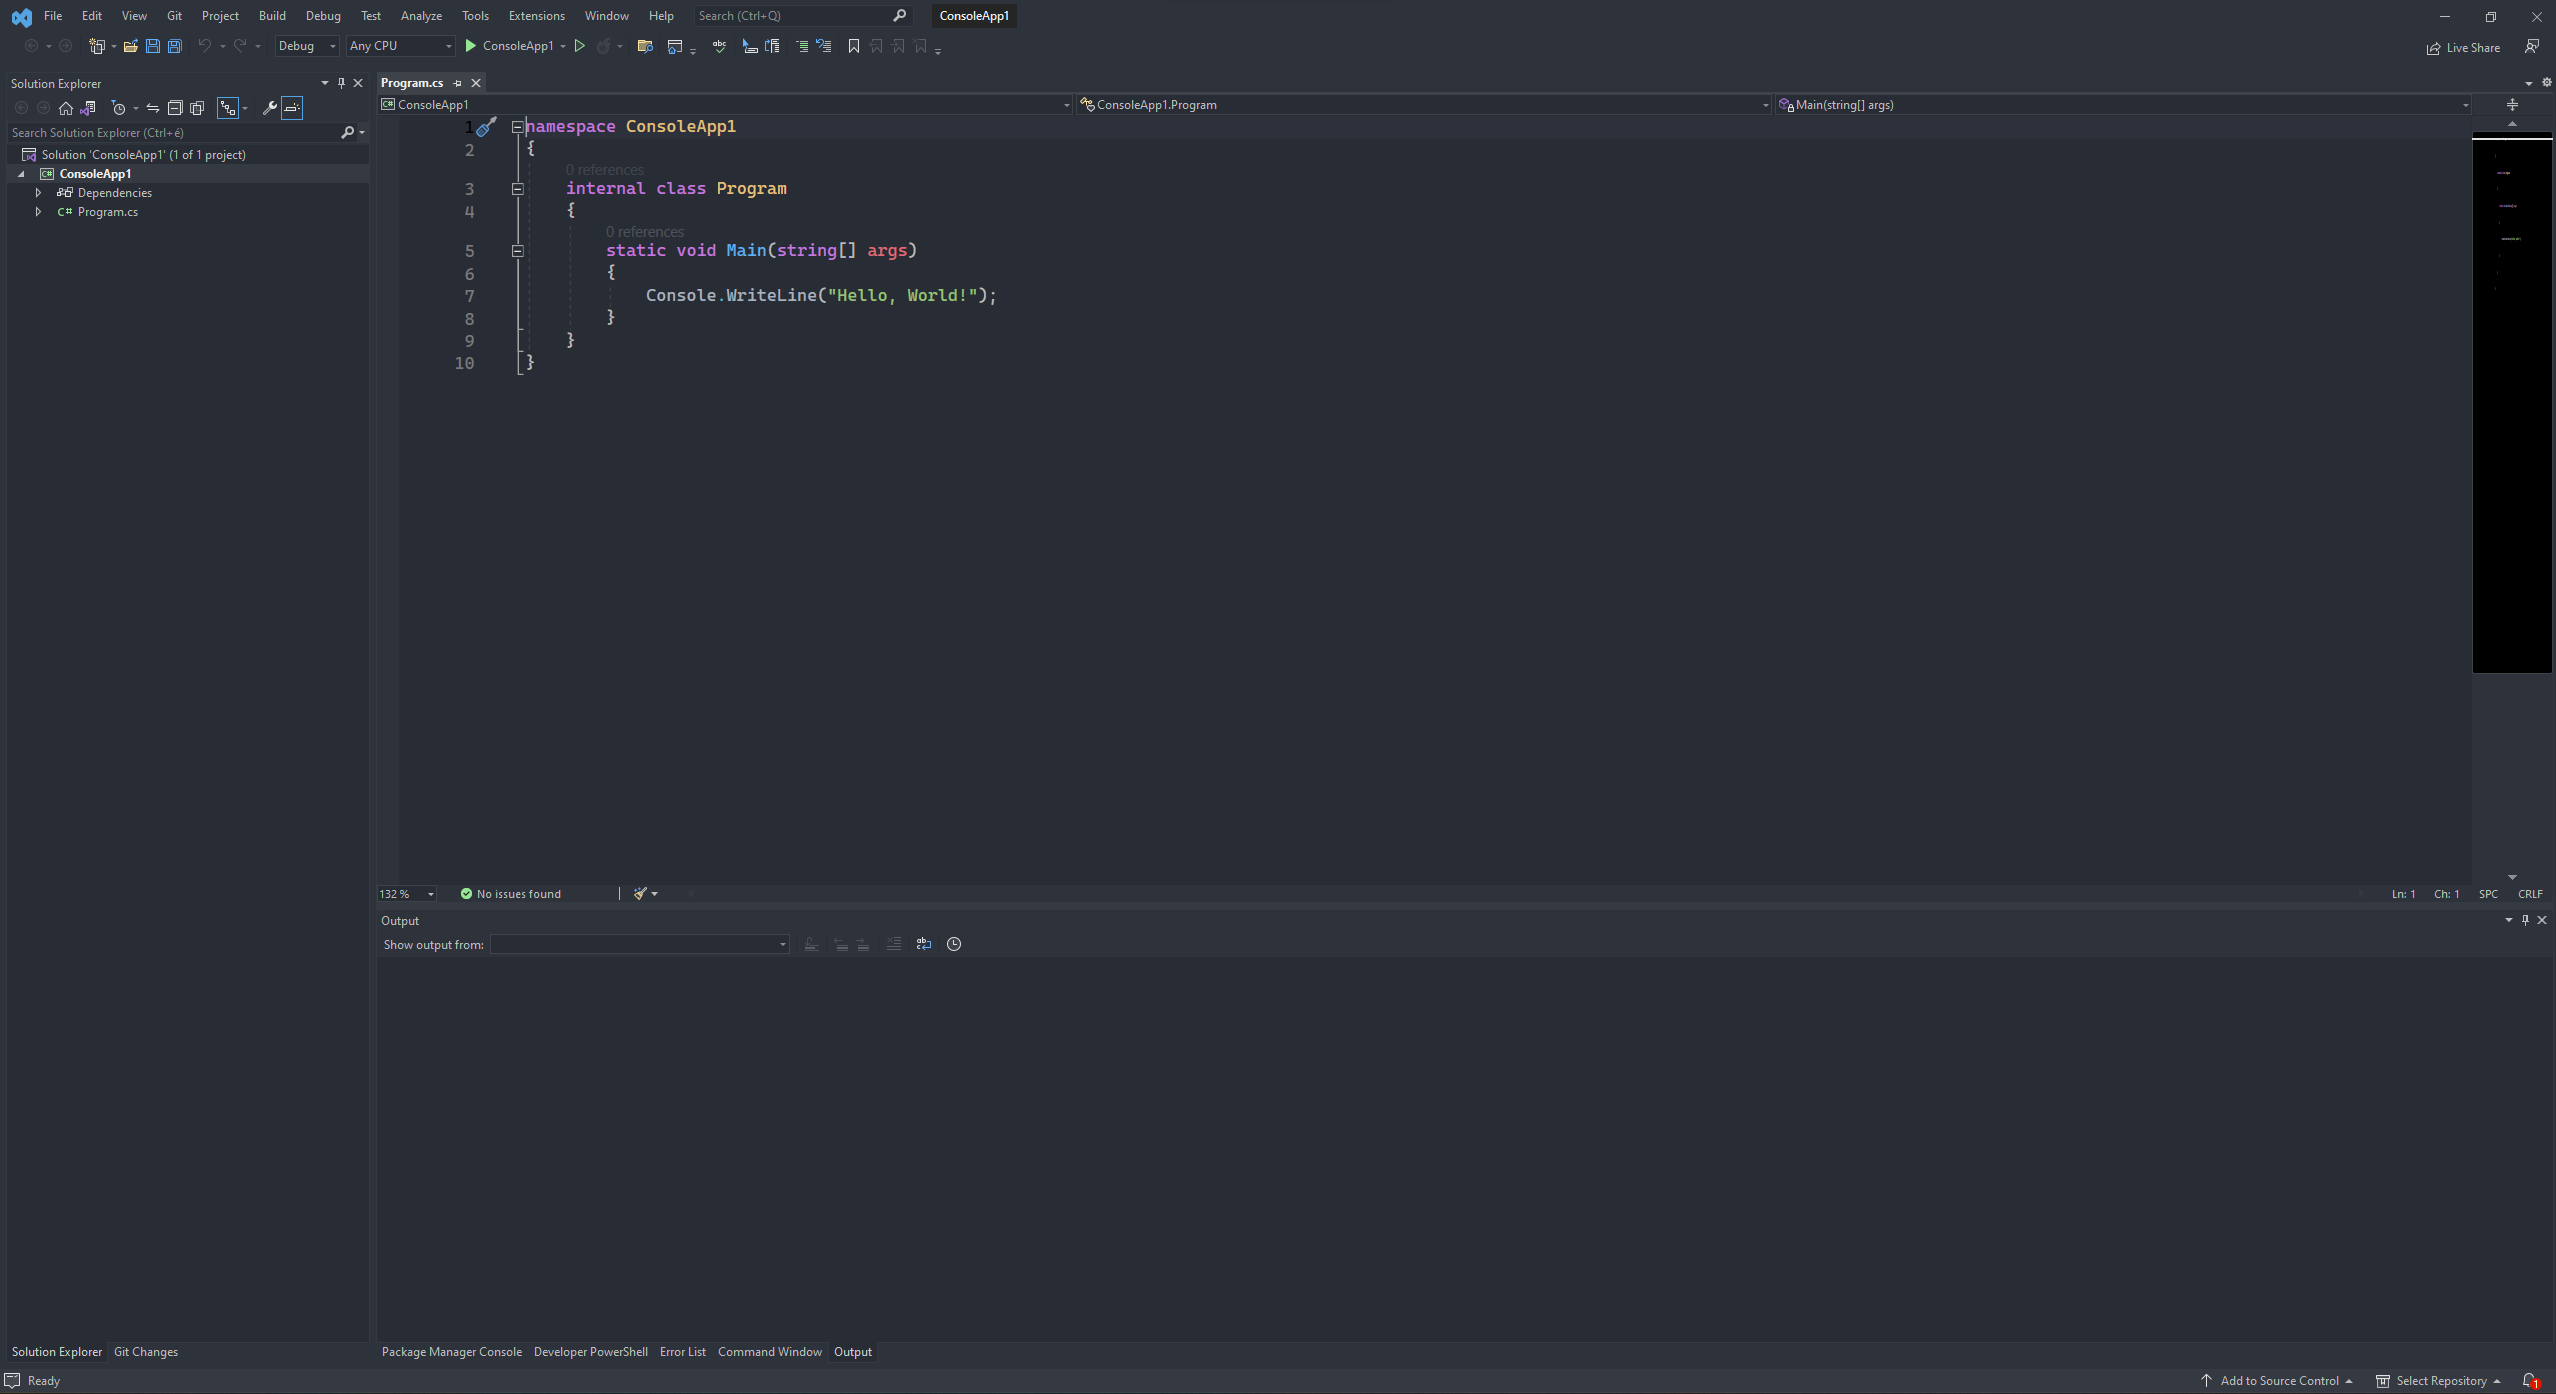
\includegraphics[width=12.0truecm]{images/VisualStuido2022.png}
    \caption{Visual Studio 2022}
    \label{fig:VisualStuido2022}
\end{figure}
Míg a Visual Studio elsősorban a Windows operációs rendszerre lett tervezve, a Microsoft kiadott egy könnyebb, keresztplatformos változatot is, a Visual Studio Code-ot. Ez utóbbi támogatja a Linux és macOS operációs rendszereket is, így a fejlesztők választhatnak az operációs rendszerüknek legmegfelelőbb változat közül.

Mindkét platform lehetővé teszi az együttműködést és a csapatmunkát, és számos bővítményt és sablont kínál a gyors és hatékony fejlesztés érdekében.
%biblatex verzió
%a bibintoc heading stílussal megjelenik a tartalomjegyzékben, title-lel a megjelenő címsor szövege módosítható
\printbibliography[heading=bibintoc,%
    title=Források]
%sima bibtex verzió
%\bibliographystyle{plain}
%\bibliography{dolgozat.bib}

\pagestyle{empty}

\section*{CD Használati útmutató}

\subsection*{Mappa szerkezet}
\dirtree{%
	.1 document/.
	.2 chapters/.
	.2 cover/.
	.2 images/.
	.2 styles/.
	.2 dolgozat.pdf.
	.1 watchwithfriends\_client/.
	.2 src/.
        .2 public/.
        .1 WatchWithFriends\_Backend/.
        .2 WatchWithFriends\_Backend/.
        .3 Services/.
        .3 Models/.
        .3 Middleware/.
        .3 Controllers/.
        .3 Hubs/.
        .3 Extensions/.
        .2 WatchWithFriends\_Data/.
        .3 Data/.
        .3 Extensions/.
        .3 Migrations/.
        .3 Models/.
        .3 Repositories/.
        .2 WatchWithFriends\_uTests/.
        .1 README.md.
}
\vspace{2em}
\subsection*{document}
Ez a könyvtár tartalmazza a szakdolgozathoz kapcsolódó összes fájlt, beleértve magát a szakdolgozatot is.

\begin{itemize}
\item \texttt{chapters:} Tartalmazza a fejezeteket.
\item \texttt{cover:} A borítók mappája.
\item \texttt{images:} A szakdolgozatban felhasznált képek.
\item \texttt{styles:} A szakdolgozatban alkalmazott stílusok.
\item \texttt{dolgozat.pdf:} A szakdolgozat PDF formátumban.
\end{itemize}

\subsection*{watchwithfriends\_client}
Ez a könyvtár tartalmazza a kliens fájlokat.

\begin{itemize}
\item \texttt{src:} A kliens forrásfájljai.
\item \texttt{public:} Különböző assetek tárolója.
\end{itemize}

\subsection*{WatchWithFriends\_Backend}
Ez a könyvtár tartalmazza a backend-hez kapcsolódó összes fájlt.

\subsubsection*{WatchWithFriends\_Backend}
Itt találhatóak az összes üzleti logikával kapcsolatos fájlok.

\begin{itemize}
\item \texttt{Services:} Az üzleti logikát végrehajtó forrásfájlok.
\item \texttt{Models:} A backenden használt modellek és DTO-k.
\item \texttt{Middleware:} A middleware által használt metódusok.
\item \texttt{Controllers:} Az összes végpontot tartalmazó mappa.
\item \texttt{Hubs:} A hubokat és az azokhoz tartozó interfészeket tartalmazza.
\item \texttt{Extensions:} Különböző bővítmény metódusokat tartalmaz.
\end{itemize}

\subsubsection*{WatchWithFriends\_Data}
Ez a könyvtár tartalmazza az adatbázissal kapcsolatos metódusokat, migrációkat és modelleket.

\begin{itemize}
\item \texttt{Data:} Az adatbázis kontextusokat tartalmazza.
\item \texttt{Extensions:} Különböző bővítmény metódusokat tartalmaz.
\item \texttt{Migrations:} A migrációkat tartalmazza.
\item \texttt{Models:} Az adatbázisban szereplő táblák modeljeit tartalmazza.
\item \texttt{Repositories:} Az adatbázishoz kapcsolódó osztályokat tartalmazza.
\end{itemize}

\subsubsection*{WatchWithFriends\_uTests}
Ez a könyvtár tartalmazza a unit teszteket.

\subsection*{README.md}
Ez a fájl tartalmazza a program futtatásához szükséges leírást.

\end{document}
